
\section{Requirements and System Model}\label{sec:requirements}
Big data is highly dependent on cloud-edge computing, which makes extensive use of multitenancy.
Multitenancy permits sharing one instance of infrastructures, platforms or applications by multiple tenants to optimize costs.
This leads to common scenarios where a service provider offers subscription-based analytics capabilities in the cloud,
or a single data lake is accessed by multiple customers.
Thus, it is a common situation to have a big data pipeline where data and services belong to various organizations,
posing a serious risk of potential privacy and security violation.
In the following of this section,
we present our system model (Section \ref{sec:systemmodel}),
the requirements driving our work (Section \ref{sec:accesscontrol_req}),
and our reference scenario (Section \ref{sec:reference}).
\AG{
  The fundamental concept underlying our methodology is to enhance the prevailing paradigm for big data pipelines through the creation of a Data Governance framework tailored to contemporary data-driven pipelines.
  The primary objective of this framework is to facilitate the assembly of data processing services, with a central focus on the selection of these services to optimize data quality, all while upholding privacy standards.
}
\subsection{Motivations}
\subsubsection{Background}
\subsubsection{Data Protection}
Research on data governance and protection focuses on the definition of new approaches and techniques aimed to protect the security and privacy of big data (e.g., CIA triad), as well as managing their life cycle with security and privacy in mind. Often, the research community is targeting specific security and privacy problems, resulting in a proliferation of solutions and tools, which are difficult to integrate in a coherent framework. Many solutions have been developed to protect the users' identity (e.g., anonymity \cite{wallace1999anonymity}, pseudonimity \cite{pfitzmann2001pseudonymity}, k-anonymity \cite{k-anon}), to guarantee data confidentiality and integrity (e.g., encryption \cite{thambiraja2012survey}, differential privacy \cite{hassan2019differential}, access control \cite{tolone2005access,servos2017current}), and to govern data sharing and analysis (e.g., data lineage \cite{woodruff1997supporting}, ETL/ELT ingestion \cite{vassiliadis2009survey}).

This project proposal focuses on access control, an approach adopted to protect access to data from unauthorized users from the very beginning of ICT systems. Coming to big data, most of the current solution leverage on Attribute-Based Access Control (ABAC) \cite{NIST:ABAC:2014} to manage policy rules adaptable at run time using attributes. In general, these systems must be instantiated on the specific scenario of interest and are ineffective when complexity increase due to the computational overhead and introduction of delays in policy enforcement. There are also database-centric approaches that focus on specific databases such as noSQL databases or graph databases, or specific types of analytical pipelines such \cite{AConGraphDB:2021, AConMongoDB:2022, ABACforHBase:2019}. However, these solutions are widely based on query rewriting mechanisms leading to high complexity and low efficiency. Finally, some solutions are scenario-specific (federate cloud, edge microservices or IoT) and lack the generality needed to adapt to multiple contexts \cite{MultipartyAC:2019, IoTSecurity}.
The closest approach to this project proposal is the work of Hu et al. \cite{ HUFerraiolo:2014}, introducing a generalized access control model for big data processing frameworks, which can be extended to the Hadoop environment. However, the paper discusses the issues only from a high-level architectural point of view, without discussing a tangible solution. Another relevant work is by Xue et al. \cite{GuardSpark:ACSAC:2020}. They propose a solution based on the notion of purpose-aware access control \cite{Byun2008} that, although focusing only on Apache Spark, recognizes the need of a generalized approach to deal with access control in analytics pipelines.

An effective data governance and protection approach cannot avoid its integration within state-of-the-art big data infrastructures. In fact, as organizations see practical results and significant value in the usage of big data, they also recognize the limits of current big data ecosystems with respect to data governance and data protection. Recently, both industry and academic communities started to investigate the issue, both from a data governance perspective \cite{al2018exploring,aissa2020decide} or recognizing the need of new security requirements \cite{Colombo:JournCybersec:2019}. Although Attribute Based Access Control (ABAC) \cite{NIST:ABAC:2014} is currently adopted in big data projects as a common underlying model given its ability to support highly flexible and dynamic forms of data protection to business-critical data, the dynamic and decentralized nature of big data asks for new solutions. Actual solutions are neither general nor scalable, since they are either platform-dependent or coarse-grained \cite{Colombo:JournCybersec:2019}.
%
Platform-specific approaches are designed for single systems only (e.g., MongoDB, Hadoop) and leverage on native access control features of the platform \cite{rathore2017hadoop,anisetti2018privacy}.
Some recent proposals, like Federated Access Control Reference Model (FACRM) \cite{FederationAC:Journ:2020} or \cite{Sandhu:ABAC:2018,GuptaSandu:2017}, are specifically tailored to the Apache Hadoop stack.
On the other hand, platform-independent approaches have the advantage of being more general than platform-specific solutions. However, the currently available platforms either model resources to be accessed as monolithic files (e.g., Microsoft DAC) or lack scalability.

Finally, the success of big data and the increasing central role of data in our everyday life increased the attention also by institutions and public administrations resulting in new regulations and guidelines.
%
The possibility of using data indiscriminately by analyzing and sharing them has led to the emergence of specific and stringent regulations such as the General Data Protection Regulation (GDPR)\cite{gdpr}. GDPR is the first and best known of a series of regulations that aim to achieve this goal. GDPR enforced in 2018, replaced the inadequate Data Protection Directive 95/46/EC. GDPR was intended to raise awareness of companies and consumers on security, privacy and the right to be forgotten.
%
The enormous growth of machine learning technologies and their pervasive diffusion, has led to the idea that artificial intelligence was also a field to be regulated. On 8 April 2019, the High-Level Expert Group on AI presented Ethics Guidelines for Trustworthy Artificial Intelligence, which proposes the development of reliable AI, that is: lawful, robust and ethical \cite{euai}.
%
Finally, the problem of guaranteeing data sovereignty clearly emerged and is leading EU commission activities \cite{pedreira2021review}. In this context, project Gaia-X, presented in October 2019 by the German and French Ministries of Economic Affairs, gathered more than 5,000 participants in one year. The project aims to satisfy a widespread need of European countries to regain possession of the sovereignty of their data, facilitate the creation of interconnected data spaces that comply with compliance criteria, open-source software, providing certification tools \cite{gaiax}. Another example of work on the data sovereignty topic is the development of the European Data Governance Act that is currently underway and aims to regulate and encourage data sharing within the European Union \cite{edca}.
\subsubsection{Data Processing}
The need of analyzing and extracting value from data emerged from the very beginning of ICT,
and is at the basis of a vast research area that includes database technologies \cite{palanisamy2020survey},
data mining \cite{jain2013data,castano2017exploratory},
big data analytics \cite{tsai2015big} and machine learning \cite{qiu2016survey}.
This project proposal focuses on machine learning in the context of modern big data infrastructures.
Research on machine learning focused on many aspects of data learning and analysis,
and is horizontal to multiple domains and research areas.
Machine learning has evolved from simple mining based on logistic regression and naive Bayes to Deep Learning,
via Decision tree and linear regression.
Deep learning is a subset of Neural Network techniques,
which owe their success to the ever increasing computational power and massive amount of data available.
Deep Learning copes well with the distribution of computations reaching excellent performances thanks to the work done in the parallelization of machine learning processing \cite{verbraeken2020survey, Goodfellow-et-al-2016,wu2022survey}.

At the same time, substantial research and development effort has been put on the infrastructures supporting data analysis, which underwent a gradual evolution starting from a monolithic model towards a model based on micro and nano services \cite{kratzke2018brief}. The spread of the cloud computing and  containerized systems allowed these systems to be more resilient, easier to develop, and adaptive, while increasing their complexity.\footnote{Today the Apache big data ecosystem counts more than 50 tools.}
With the spread of big data, new tools and infrastructures have been developed for data ingestion, storage, and analysis. The main challenge to be addressed was the inability for a single system to handle such huge amount of data; this resulted in the spread of solutions based on a distributed file system \cite{blomer2015survey}, a system that permits to share data across multiple machines (made in general of commodity hardware), making possible for the user to read and write data without perceiving this distribution. Over the years these systems have seen more and more refinements and expansions, such as, resource managers to manage the distribution of resources in the network of nodes (YARN) \cite{kulkarni2014survey}, SQL-Like systems that support access following standard RDBMS (HIVE, Presto, Trino) \cite{thusoo2009hive,sethi2019presto}. Finally, other software components (for example Apache Spark \cite{salloum2016big}) have been created to meet the ever increasing needs for data access and analysis requested by machine learning technologies.
\subsection{System Model}\label{sec:systemmodel}
\AG{
  In our context, a \user aims to execute a data pipeline to perform some analysis or transformation procedures on some data.
  The input data are considered alredey cleaned,
  Policies governing the data are established, which can originate from the \user, third-party entities, or regulatory frameworks.
  For instance, a policy may restrict the execution of processing operations to a specific geographic region.
  The \user is provided with a set of empty pipeline templates. Each template represents a blank pipeline with the necessary steps but without the specific services.
  The user is given the opportunity to choose, for each step of the template, from a collection of candidate services that are functionally equivalent and comply with the specified policies.
  By selecting the most suitable service template from a range of available options,
  the \user ensures an alignment between the service composition and their distinctive demands.
  These services are subsequently ranked based on their ability to retain the maximum amount of data while maintaining an equivalent level of privacy.
  Underlying our investigation is the assumption that a greater quantity of preserved data corresponds to enhanced data quality.
}

Our reference scenario is a service-based environment where services are composed according to a pipeline template.

It includes the following parties:
i) User: the entity that wants to perform some analytics on the data
ii) Pipeline: a sequence of connected services that process and move data from one point to another in a structured and automated manner.
iii) Service: a software that performs a specific task, a service is characterized by two function: the service function and the policy function.
iv) Service composition: the process of combining two or more services to create a new service
v) Policy: a structured set of guidelines, rules, and procedures that define how the service must safeguards its data to maintain confidentiality
% \begin{itemize}
%   \item User owns some data and wants to perform some analytics on it
%   \item Choose a pipeline template and a wanted level of privacy
%   \item The template has lambda, signed
%   \item Policy is a set of rules
%   \item Match the policy with the lambda
%   \item Compares services that match the policy ranking them based on quality
%   \item Choose the best service
%   \item The composite service is executed
% \end{itemize}

\AG{
  The rise in data production has led the scientific community to split into two main areas of focus.
  On one side, researchers are working on ways to make the most of the valuable data we have.
  On the other side, there's a growing need to keep data safe and private.
  These two directions are happening at the same time, but there are not many solutions that find a good balance between them.
  So, the solution we propose aims to create a framework that can strike a balance between privacy and data quality.
  We want to get as much quality from the data as possible while still protecting privacy.
  Our system model aims to achieve an optimal service composition to ensure privacy and data quality.
  Within this context, we contemplate an interconnected sequence of services, establishing a pipeline where individual nodes signify distinct services.
  Each stage within the pipeline undertakes the task of data transformation or processing, with the resulting output serving as the input for the subsequent service.
  This model encapsulates what we refer to as a template, visually presented in Figure \ref{fig:service_composition_template}.
  In order to instantiate the template, the selection of services to be executed at each step of the pipeline becomes imperative.
  At each step, there exists a set of functionally equivalent candidate services (\s{0}\dots\s{n}) that differ in terms of annotation and data transformation.
  These services are annotated with a set of requirements that encompass crucial details
  The annotations play a pivotal role in the creation of policies that determine the eligibility of a service for deployment.
  By enforcing such policies, the set of candidate services for a given step is reduced.
  The remaining services undergo evaluation based on their potential impact on the data transformation process.
  Preference is given to the service that maximizes data quality while ensuring an equal level of data privacy.
  This evaluation process aids in identifying the most suitable service for a particular step in the pipeline.
  Upon the selection of the most appropriate service for each step, the instantiation of the pipeline is deemed complete.
  Consequently, the pipeline becomes ready for execution, with the assurance that the chosen services align with the specified requirements and optimize the desired outcomes.
}

\subsection{Reference Scenario}
Our reference scenario is a service-based environment where services are composed according to a pipeline template.
Our case study is grounded in the analysis of a dataset comprising individuals held in Department of Correction facilities in the state of Connecticut while awaiting trial.
The dataset\footnote{https://data.ct.gov/Public-Safety/Accused-Pre-Trial-Inmates-in-Correctional-Faciliti/b674-jy6w}, exhibits a straightforward row-and-column structure.
Each row represents an inmate, and the columns include the following attributes: date of download, a unique identifier, last entry date, "race," gender, age of the individual, the bound value, offense, entry facility, and detainer.
To serve the objectives of our study, we have extended this dataset by introducing randomly generated first and last names.

Within the context of our case study, we envision the establishment of a service pipeline designed as follows:
The end user, a member of the Connecticut Department of Correction (DOC),
seeks to perform an analysis on the dataset to compare admission trends in Connecticut prisons with those in other states.
The user's preferences align with a predefined template that orchestrates the following sequence of operations:
i) Anonymization of the dataset.
ii) Expansion of the dataset, integrating data from the states of New York and New Hampshire.
iii) Transformation of the dataset to derive state-specific data aggregations, including statistical measures like averages, medians, and clustering-based statistics.
iv) Storage of the resultant data in reference states. Specifically, one copy remains in Connecticut (where sensitive information in the source dataset is not protected), while two additional copies are distributed to New York and New Hampshire (with sensitive information from the source dataset being safeguarded).

It is important to note that the template mandates that the entire service is executed within a single country, and any instance where the data must traverse beyond the boundaries of Connecticut, rigorous data protection measures are implemented.
A visual representation of the template is presented in Figure \ref{fig:service_composition_example}.

At each service you can see examples of the use of the f and lambda functions.
In the first step That of anonymization the service f is empty since the service does not apply any transformation.
The anonymization is in fact borne by the policy via the \myLambda function.
In the second step of expansion the function is adoptive in that it extends the dataset by merging it with other sources, the policy instead only enforces execution on Connecticut territory.
In the third step the transformation one the Function is transformational in that it aggregates the data to extract statistics from it the policy is the same as in step 2, finally in the last step the transformation F is empty in that the service only stores the dataset.
The policy instead performs an anonymization just on the geolocation


\begin{figure}
  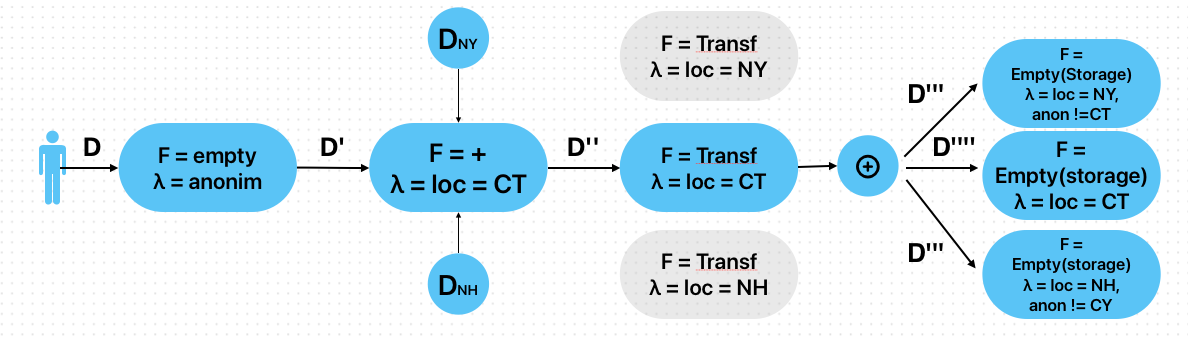
\includegraphics[width=0.98\columnwidth]{service_composition_example}
  \caption{Service composition example.}\label{fig:service_composition_example}

\end{figure}



\section{Service}
\subsection{Service Definition}

A service is defined as a graph. G(V, E, F)

\subsection{Service Flow}
Within the framework, a service is defined as an entity that receives input data, processes it by applying a transformation function, and produces an output result. Each service essentially consists of two parts:
\begin{enumerate}
  \item The service transformation function (\Transformation{F}{\myGamma}).
  \item The policy transformation function (\Transformation{P}{\myLambda}).
\end{enumerate}
Where \myGamma and \myLambda are instrumentations of the service. That is, the service is tagged with \myLambda and \myGamma.

The execution of a service can be conceptually divided into 4 phases:
\begin{enumerate}
  \item Policy enforcement: The framework applies the service policy (\Transformation{P}{\myGamma})
        to the data. This may typically involve transforming or filtering the dataset.
  \item Data reception: The service receives input data from the user or from the service preceding it in the workflow. The received data is averaged by the framework via application of the previous step. The data that the service receives is therefore to be considered privacy ready.
  \item Service function execution: The Service applies its processing function. The function can be of 4 main types:
        \begin{itemize*}
          \item \F{Empty} The function applies no transformation or processing on the data.
          \item \F{additive} The function expands the amount of data received, for example, by integrating it with data from other sources.
          \item \F{transformation} The function transforms some records in the dataset without altering the domain.
          \item \F{domain change }  The function changes the domain of the data by applying e.g. PCA or Kmeans (will not be considered in the current work).
        \end{itemize*}
  \item Calculation of metrics $\rightarrow$ The framework calculates the quality metrics on the dataset produced downstream of the application of the function.
\end{enumerate}
Output of the result $\rightarrow$ the obtained dataset is brought to the output.


In essence, the execution of a service can be conceptualized as a multi-stage process, wherein input data is received, subjected to a defined function, quality metrics are assessed, policy is applied, further metrics are computed, and the ultimate result is readied for further application or analysis.
% We formally model a Big Data analytics pipeline as follows.

% \begin{definition}[Big Data Analytics Pipeline] \label{def:pipeline}
%   A Big Data Analytics pipeline \G(\V,\E) is a direct acyclic graph having a root \vi{r}$\in$\V, a vertex \vi{i}$\in$\V$_I$$\subseteq$\V\ for each job \job{i} invocation, two additional vertices \vi{c},\vi{m}$\in$\V$_{\otimes}$$\subset$\V\ for each alternative ($\otimes$) structure modeling the alternative execution (\emph{choice}) of operations and the retrieval (\emph{merge}) of the results,
%     respectively, and two additional vertices \vi{f},\vi{j}$\in$\V$_{\oplus}$$\subset$\V\ for each parallel ($\oplus$) structure modeling the contemporary execution (\emph{fork}) of operations and the integration (\emph{join}) of their results, respectively.
% \end{definition}

% We note that each vertex \vi{i} model a job \job{i} provided by an organization \org{i}.
% We also note that an analytics pipeline can be deployed following a centralized or a decentralized approach as discussed in detail in Section \ref{sec:architecture}.

\begin{figure}[!t]
  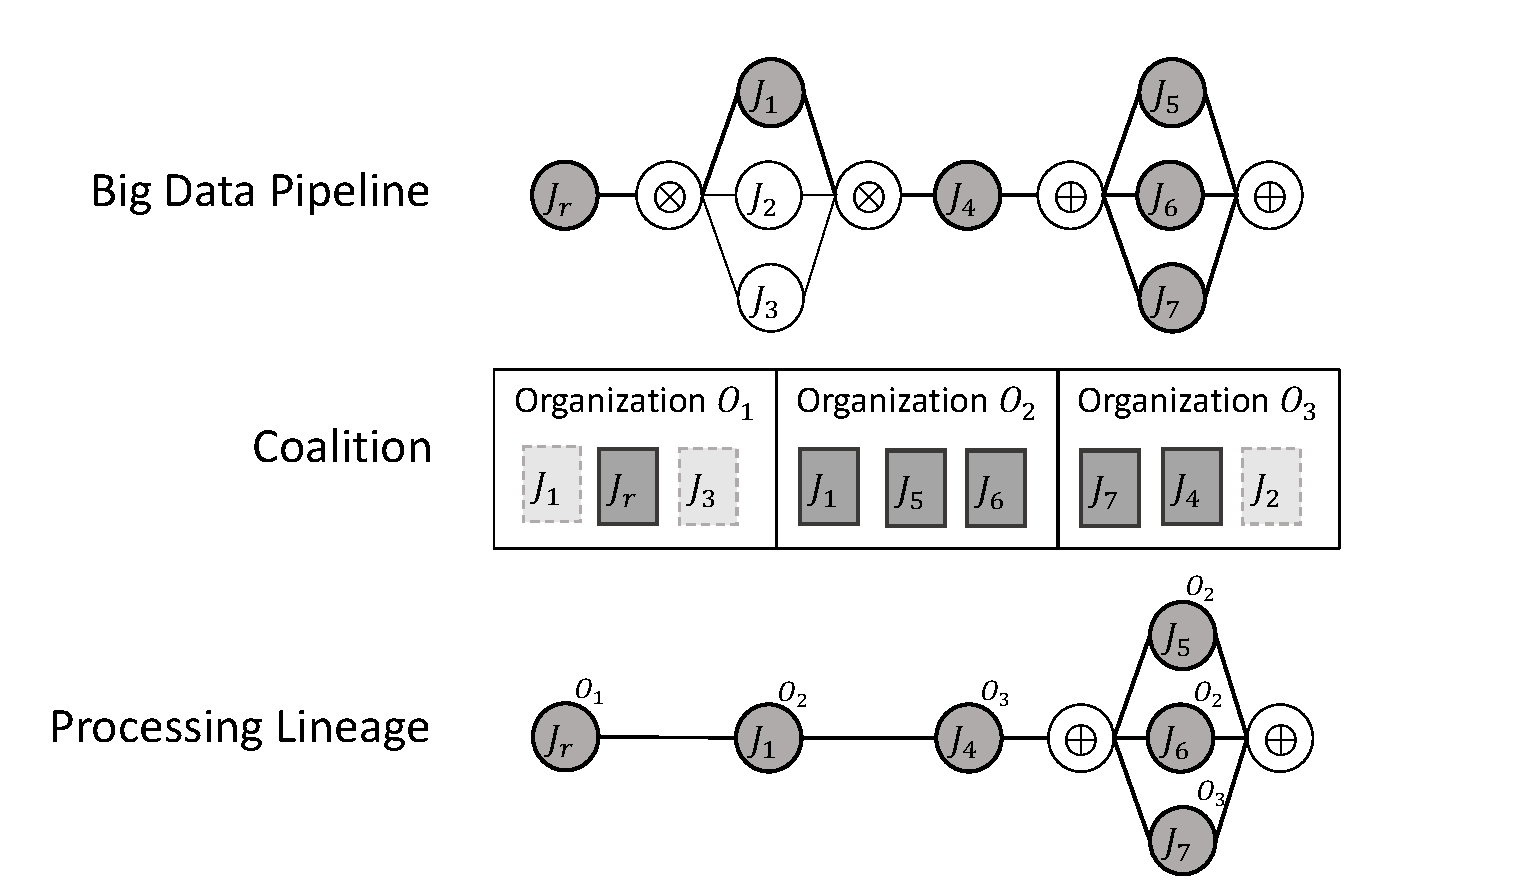
\includegraphics[width=0.98\columnwidth]{generaleFig1.pdf}
  \caption{Big Data Analytics pipeline graphs with a coalition of organization for a given processing lineage.}\label{fig:BDpipeline}
\end{figure}

Figure~\ref{fig:BDpipeline} shows an overview of our system model.

%Solid arrows present the typical batch or analytics model generation flows. Dashed arrows present typical streaming or prediction flows. \CH{togliere dalla figura la linea che separa le due procedure e le scritte ingestion procedure e analytics procedure?}
%The coalition creation is driven by missions including emergency and disaster management, humanitarian operations, or simply interdependent organizations.
%\CH{Qui ho introdotto solo il termine coalition, va spiegato anche il termine federation?}





\section{Service Template}
\subsection{Definition}
The main point of our investigation is a service-based environment where services are combined strategically with policies that cater to the specific needs of the user.
Our focus is on service composition, which involves three main actors and operates at a higher level of abstraction.
\begin{enumerate}
  \item The \User:
        The stakeholder within the service-based environment,
        the \user assumes the role of the entity initiating the request for a particular service.
        By choosing a template, the \user initiate the subsequent stages of the composition process.
  \item The Service Template:
        At the crux of effective service composition lies the pivotal role played by the service template.
        Functioning as a high-level composition of services labeled with predefined policies,
        the service template serves as a structured blueprint facilitating the decision-making process for the  \user.
        \begin{definition}[Service Template] \label{def:pipeline}
          A Service Template \T(\V,\E,$\iChartFunction{}$), is a direct acyclic graph having a root \vi{r}$\in$\V, a vertex \vi{i}$\in$\V\ for each service $s_i$,
          two additional vertices \vi{c},\vi{m}$\in$\V$_{\timesOperator}$$\subset$\V\ for each alternative ($\timesOperator$) structure modeling the alternative execution (\emph{choice}) of operations and the retrieval (\emph{merge}) of the results,
                respectively, and two additional vertices \vi{f},\vi{j}$\in$\V$_{\plusOperator}$$\subset$\V\ for each parallel ($\plusOperator$) structure modeling the contemporary execution (\emph{fork}) of operations and the integration (\emph{join}) of their results, respectively. $\iChartFunction{}$ is an annotation function, assigning to each vertex \vi{i}$\in$\V\ a set of policies \Pset{i}.
        \end{definition}
        % We note that $\{$\vi{r}$\}$ $\cup S_\timesOperator\cup S_\plusOperator=S$\\
  \item The Service Provider:
        Central to the execution of service composition is the service provider,
        serving as the responsible entity for delivering the requested service.
        Tasked with adhering to the prescribed service template, the service provider execute the service requested by the \user.
\end{enumerate}

% More detail about the structure modeling the alternative and parallel follows :

% \textbf{Sequence} ($\plusOperator$). It composes two service, $wsi$ and $wsj$, in a sequence. $wsi\plusOperator wsj$ mimics a composition where $wsj$ is executed after $wsi$.

% \textbf{Alternative} ($\timesOperator$). It composes two service, $wsi$ and $wsj$, in an alternative. $wsi\timesOperator wsj$ mimics a composition where either $wsi$ or $wsj$ is executed.

% \textbf{Parallel} ($\plusOperator$). It composes two service, $wsi$ and $wsj$, in parallel. $wsi\plusOperator wsj$ mimics a composition where both $wsi$ and $wsj$ are executed simultaneously.
\begin{figure}[h!]
  \centering
  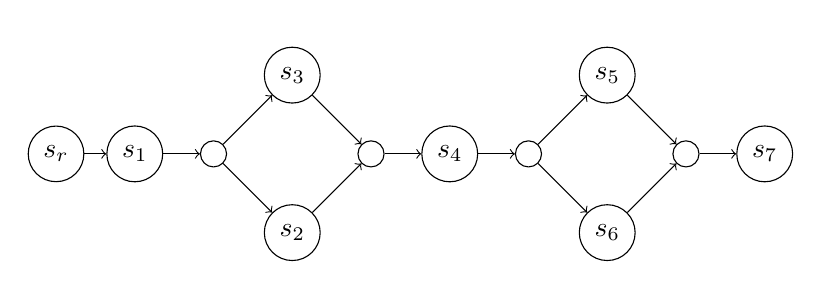
\begin{tikzpicture}
    % Nodes
    \node[draw, circle] (node1) at (0,0) {$s_r$};
    \node[draw, circle] (node2) at (1,0) {$s_1$};
    \node[draw, circle] (node3) at (2,0) {$\timesOperator$};
    \node[draw, circle] (node4) at (3,-1) {$s_2$};
    \node[draw, circle] (node5) at (3,1) {$s_3$};
    \node[draw, circle] (node6) at (4,0) {$\timesOperator$};
    \node[draw, circle] (node65) at (5,0) {$s_4$};
    \node[draw, circle] (node7) at (6,0) {$\plusOperator$};
    \node[draw, circle] (node8) at (7,1) {$s_5$};
    \node[draw, circle] (node9) at (7,-1) {$s_6$};
    \node[draw, circle] (node10) at (8,0) {$\plusOperator$};
    \node[draw, circle] (node11) at (9,0) {$s_7$};
    % Text on top
    \node[above] at (node1.north)  {$\tChartFunction$};
    \node[above] at (node2.north)  {$\tChartFunction$};
    \node[above] at (node3.north)  {                 };
    \node[above] at (node4.north)  {$\tChartFunction$};
    \node[above] at (node5.north)  {$\tChartFunction$};
    \node[above] at (node65.north) {$\tChartFunction$};
    \node[above] at (node8.north)  {$\tChartFunction$};
    \node[above] at (node9.north)  {$\tChartFunction$};
    \node[above] at (node11.north) {$\tChartFunction$};
    % Connection
    \draw[->] (node1) -- (node2);
    \draw[->] (node2) -- (node3);
    \draw[->] (node3) -- (node4);
    \draw[->] (node3) -- (node5);
    \draw[->] (node5) -- (node6);
    \draw[->] (node4) -- (node6);
    \draw[->] (node6) -- (node65);
    \draw[->] (node65) -- (node7);
    \draw[->] (node7) -- (node8);
    \draw[->] (node7) -- (node9);
    \draw[->] (node8) -- (node10);
    \draw[->] (node9) -- (node10);
    \draw[->] (node10) -- (node11);
  \end{tikzpicture}
  \caption{Service composition template}
  \label{fig:service_composition_template}
\end{figure}

\subsection{Policy}
% \subsubsection{Annotations}
% \subsubsection{Transformation}

\subsubsection{Policy Decision/Policy Matching}
\subsubsection{Policy Enforcement}
\subsubsection{Policy Evaluation}